\documentclass[a4paper,12pt]{report}
%general packages
\usepackage[T2A]{fontenc}
\usepackage[utf8]{inputenc}
\usepackage[english,russian]{babel}
\usepackage{circuitikz}
\usepackage{wrapfig}
\usepackage{makecell}
\usepackage{tabularx}
\usepackage{graphicx}
\usepackage{gensymb}
\usepackage{cancel} %cancel symbol
\usepackage{amsmath,amsfonts,amssymb,amsthm,mathtools}
\usepackage[dvipsnames]{xcolor}
\usepackage{subcaption}

%fancy header + geometry
\usepackage{fancyhdr}
\usepackage[a4paper,includehead,nomarginpar,left=15mm,right=15mm,top=15mm,headheight=10mm,bottom=20mm]{geometry}

%pgfplots
\usepackage{pgfplots}
\usepackage{pgfkeys}
\pgfplotsset{compat=1.12}
\usepackage{mathrsfs}

%multi column text
\usepackage{blindtext}
\usepackage{multicol}

%tikz (draw)
\usepackage{tikz}
\usepackage{pstricks-add}
\usetikzlibrary{intersections}
\usetikzlibrary{arrows.meta}
\usetikzlibrary{calc,angles,positioning}
\usetikzlibrary{arrows}
\usepackage{float}

%parskip settings
\parindent=0ex
\setlength{\parskip}{\baselineskip}%
\setlength{\parindent}{0pt}%

%fancy notation for sets
\newcommand{\R}{{\mathbb R}}
\newcommand{\N}{{\mathbb N}}
\newcommand{\fancy}[1]{{\mathbb{#1}}}
%sgn function
\DeclareMathOperator{\sgn}{sgn}

% intersection and union symbols
\newcommand{\uni}{\cup}
\newcommand{\inter}{\cap}
\newcommand{\re}{\text{Re}}
\newcommand{\const}{\text{const}}

\renewcommand{\footrulewidth}{0.4pt}

%\newcommand{\celsius}{$\ ^\circ C$}

%environments

\newlength{\twosubht}
\newsavebox{\twosubbox}

\newtheorem{problem}{Задача}[]
\newenvironment{sol}{\paragraph{Решение}}{}
\renewcommand\thesection{\arabic{section}}

\usepackage{titlesec}
\titlespacing*{\section}
{0cm}{\baselineskip}{0pt}
\titlespacing*{\subsection}
{0pt}{0.1\baselineskip}{0.1\baselineskip}
\titlespacing*{\paragraph}
{0pt}{0.1\baselineskip}{\baselineskip}

\setcounter{secnumdepth}{0}

\begin{document}
	

\begin{titlepage}
	\begin{center}
		МОСКОВСКИЙ ФИЗИКО-ТЕХНИЧЕСКИЙ ИНСТИТУТ (НАЦИОНАЛЬНЫЙ ИССЛЕДОВАТЕЛЬСКИЙ УНИВЕРСИТЕТ) \\
		
		
		\hfill \break
		Факультет обшей и прикладной физики\\
		\vspace{2.5cm}
		\large{\textbf{Отчёт по лабораторной работе 1.2.5 <<Исследование прецессии уравновешенного гороскопа>>}}\\
		\hfill \break
		\\
	\end{center}
	
	\begin{flushright}
		Выполнил:\\
		Студент гр. Б02-304\\
		Головинов. Г.А.
	\end{flushright}
	
	\vspace{7cm}
	
	\begin{center}
		
\includegraphics[width=0.15\linewidth]{uni}
	\end{center}
	

	

	\vfill
	
	\begin{center} Долгопрудный, 2023 \end{center}
	
	\thispagestyle{empty}
	
\end{titlepage}


	\newpage
	%\pagenumbering{arabic}
    %\pagestyle{fancy}

    %\fancyhead{}
    %\fancyfoot{}
    %\fancyhead[L]{\rightmark}
    %\fancyhead[R]{\thepage}
    %\fancyfoot[R]{Моделирование давление в шине при прохождении поворотов.}

    \section*{Аннотация}
        \paragraph*{Цель работы:} 1) составить и решить в общем виде задачу, которая может позволить определить изменение давления в шине автомобиля; 2) используя реальные физические размеры и зависимости температур резины определить изменение давления в разных ситуация; 3) сравнить полученные значения с другими моделями.
    \vspace{0.5cm}
    \hrule
    \section{Формулировка задачи и решение в общем виде}
    %\begin{multicols}{2}
        Мы хотим по известным начальным температурам $T_1$ и $T_2$, конечным температурам $T_1'$ и $T_2'$ и начальному давлению $p_0$ научиться находить установившееся давление $p$.

        Попробуем некоторым способом связать $p$ и $p_0$. Например, можно воспользоваться сохранением массы воздуха в шине. Тогда
        \begin{gather}
            m_0=\int \rho dV = \int_{r_1}^{r_2} \frac{p_0\mu}{RT(r)}2\pi r  D dr =\int_{r_1}^{r_2}\frac{p\mu}{RT'(r)}2\pi r D dr. 
        \end{gather}
        Здесь мы обозначили $D$ --- ширина колеса, $T(r),\ T'(r)$ --- зависимости температуры от радиуса в начальном и конечном состоянии.

        Теперь много слева и справа сокращается, получим выражение $p(p_0)$:
        \begin{equation}
            \label{p}
            p=p_0\left(\int_{r_1}^{r_2}\frac{rdr}{T(r)}/\int_{r_1}^{r_2}\frac{rdr}{T'(r)}\right).
        \end{equation}
        В принципе, это мы бы смогли проинтегрировать и получить желаемый результат, если бы у нас были зависимости $T(r)$ и $T'(r)$. Получим эти зависимости.

        Будем считать коэффициент теплопроводности $\varkappa \sim T^n$, где $n>0$. Сейчас это несколько усложнит наши подсчеты, однако потом мы сможем сразу поменять параметр $n$, если это будет необходимо.

        Тогда закон Фурье имеет вид:
        \begin{equation}
            \label{fourier}
            q=-\varkappa\frac{dT}{dr}=-AT^n\frac{dT}{dr}.
        \end{equation}
        В нашем приближении распределение температур стационарное, поэтому \begin{equation}
            Q=qS=q\cdot 2\pi r D = \text{const}, \quad \forall r\in[r_1,r_2].
        \end{equation}
        Разделим переменные в \eqref{fourier} и проинтегрируем сначала от $r_1$ до $r_2$, а потом от $r_1$ до произвольного $r$, чтобы получить $T(r)$.
        \begin{gather}
            -\frac{Q}{2\pi D A}\int_{r_1}^{r_2}\frac{dr}{r}=\int_{T_1}^{T_2}T^n dT, \quad B:=\frac{Q}{2\pi D A},\\
            -B\ln \frac{r_2}{r_1}=\frac{1}{n+1}(T_1^{n+1}-T_2^{n+1}).
        \end{gather}
        Для произвольного $r$:
        \begin{gather}
            -B\ln \frac{r}{r_1}=\frac{1}{n+1}(T^{n+1}(r)-T_1^{n+1}),\\
            T(r)=\left[\left(\ln \frac{r}{r_1}/\ln \frac{r_2}{r_1}\right)(T_2^{n+1}-T_1^{n+1})+T_1^{n+1}\right]^{\frac{1}{n+1}}
        \end{gather}
        Для $T'(r)$ просто воспользуемся уже полученным результатом для $T(r)$ и поставим в нужных местах штрихи.

    \section{Первичная проверка результатов}
        Перед тем как продолжить, стоит проверить результат на математическую и физическую корректность. Это можно сделать, например, построив графики $T(r)$, проверить выполняются ли граничные условия, сравнить форму графика с известными результатами.

        \begin{figure}[H]
            \centering
            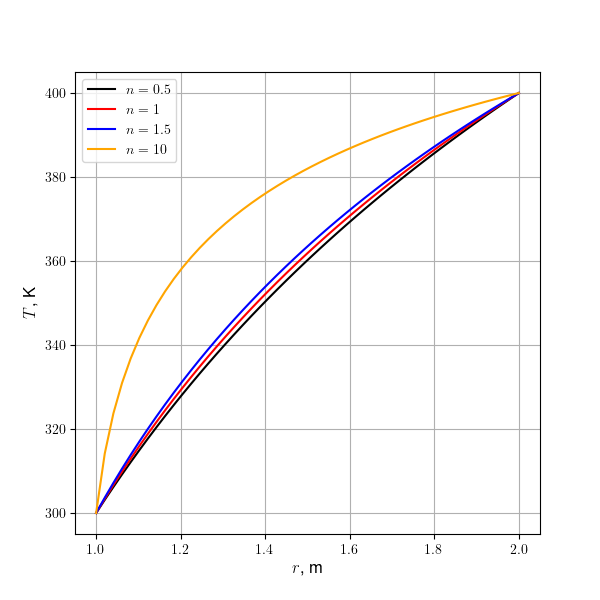
\includegraphics[width=0.7\linewidth]{img/example.png}
            \caption{Зависимость $T(r)$ при $T_1=300$, $T_2=400$, $r_1=1$, $r_2=2$ и различных $n>0$}
        \end{figure}

        Как видно, граничные условия действительно выполняются, а форма графика действительно схожа с известными результатами.

        Вторую проверку можно сделать с помощью уравнения теплопроводности. Так как $T(r)$ мы находили из условия стационарности, то наша функция $T(r)$ должна обращать уравнение теплопроводности в ноль:
        \begin{gather}
            \frac{1}{r}\frac{\partial}{\partial r}\left(r\varkappa \frac{\partial T}{\partial r}\right)=0,
        \end{gather}
        это можно проверить как прямым дифференцированием, так и подставив функцию в выражение на компьютере. Убеждаемся, что $T(r)$ действительно обращает выражение в ноль, что является еще одним подтверждением корректности нашего результата.
        
    \section{Оценка применимости формулы}
        В этом разделе мы попытаемся дать некоторую оценку времени установления стационарного распределения в шине, чтобы оценить применимость нашего результата.
        %Условием стационарности в терминах этого уравнения является равенство левой части нулю.

        %Воспользуемся результатом из лабораторной работы 2.1.2 из \cite{labnik}, чтобы оценить время, необходимое для установления стационарного распределения.
        
        Скажем, что время установления стационарного распределения примерно равно времени прогрева шины от стенок. Оценку времени прогревания получим из задачи об остывании (нагревании) полупространства. Решение этой задачи не является прямой целью в нашей работе, подробное решение изложено в параграфе 56 \cite{sivukhin}. Опишем кратко задачу и решение.

        Пусть у нас есть некоторая однородная среда, которая заполняет полупространство $x\geq0$. В начальный момент времени температура всей среды равна $T_0$, а температура плоскости $x=0$ поддерживается равной $T_1\neq T_0$. Надо найти распределение $T(x,t)$ в среде в последующие моменты времени.

        Распределение температуры описывается уравнением теплопроводности, в нашем случае оно имеет вид:
        \begin{gather}
            \frac{\partial T}{\partial t}=\chi \frac{\partial^2 T}{\partial x^2},
        \end{gather}
        где $\chi$ --- коэффициент температуропроводности среды. 

        Из 6 известных нам величин $T,\ x,\ t,\ T_0,\ T_1,\ \chi$ можно составить только 3 безразмерные комбинации:
        \begin{gather}
            \frac{T}{T_0},\quad \frac{T_1}{T_0},\quad \frac{x}{\sqrt{\chi t}}.
        \end{gather}
        Для описания распределения температуры в среде необходима некоторая связь между безразмерными комбинациями. Вторая из них вообще является константой, поэтому ничего нам не дает. Тогда должно быть
        \begin{gather}
            \frac{T}{T_0}=F\left(\frac{x}{\sqrt{\chi t}}\right),
        \end{gather}
        отсюда вытекает <<автомодельное решение>>, которое использовалось в работе 2.1.2 из \cite{labnik}. Условие
        \begin{gather}
            \frac{x}{\sqrt{\chi t}}=1
        \end{gather}
        дает нам координату $x$, в которой $T\approx(T_1+T_0)/2$
        Тогда толщину уже прогретого слоя (при изменении одной граничной температуры) найти из $x^2/(\chi t)=1$, отсюда $\tau=(r_2-r_1)^2/\chi$. Применим полученную формулу для наших радиусов и получим $\tau \sim$ 10 мин. 
        
        По факту, у нас с другой стороны на прогрев работает внешний слой резины, поэтому оценку уже можно снизить как минимум вдвое, а также не обязательно ждать прогрева до среднего арифметического всего воздуха, достаточно даже половины. Тогда результат снизится до $\tau < $ 1 мин. 
        
        Поэтому в реальности время установления меньше, но этот результат мы все равно учтем, и будем использовать формулу только на больших дистанциях (как минимум несколько кругов).
    \section{Использование полученных результатов для определения\\ изменения давления}
        К сожалению, у нас нет гоночных автомобилей, которые позволили бы проверить нашу модель, а гоночные команды не любят делиться своими данными, поэтому брать их мы будем из других симуляций и сравнивать с ними. В качестве этой симуляции возьмем, пожалуй, лучшую коммерчески доступную модель гоночных автомобилей --- iRacing. Этот сервис позволяет нам протестировать нашу модель в самых разных условиях: от штормовых и холодных, до сухих и самых жарких.

        Нам необходимо получить зависимость температур внешнего и внутреннего слоя шины, это мы будем делать с помощью телеметрии, записывать которую также позволяет сервис. 
        \begin{figure}[H]
            \centering
            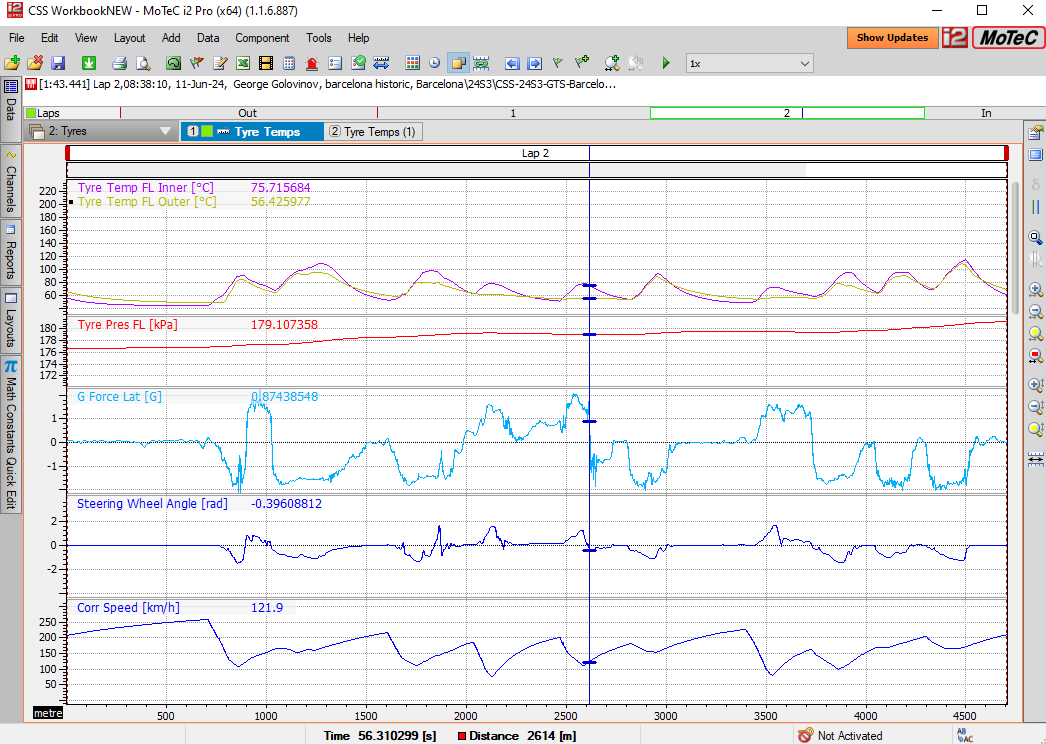
\includegraphics[width=0.7\linewidth]{img/motec_ex.png}
            \caption{Программа для анализа телеметрии MoTeC i2 Pro}
        \end{figure}
        Программа MoTeC i2 Pro используется и реальными командами для анализа телеметрии реальных гоночных автомобилей, поэтому мы максимально приблизили наше сравнение с реальностью.

        Для ясности, далее будут использоваться следующие обозначения: FL (Front Left) --- переднее левое колесо, FR (Front Right) --- переднее правое, RL (Rear Left) --- заднее левое, RR (Rear Right) --- заднее правое.

    \subsection{Тест 1}
        Первый тест прошел в относительно нормальных условиях на достаточно характерной трассе. Она имеет много правых поворотов, что создает дисбаланс между левой и правой сторонами шин. Трасса была выбрана именно из-за этой характеристики. 
        
        \begin{figure}[htp]

            % preliminary
            \sbox\twosubbox{%
              \resizebox{\dimexpr.9\linewidth-1em}{!}{%
                \includegraphics[height=4cm]{example-image-a}%
                \includegraphics[height=4cm]{example-image-16x9}%
              }%
            }
            \setlength{\twosubht}{\ht\twosubbox}
            
            % typeset
            
            \centering
            
            \subcaptionbox{Условия на трассе и другая информация\label{f}}{%
              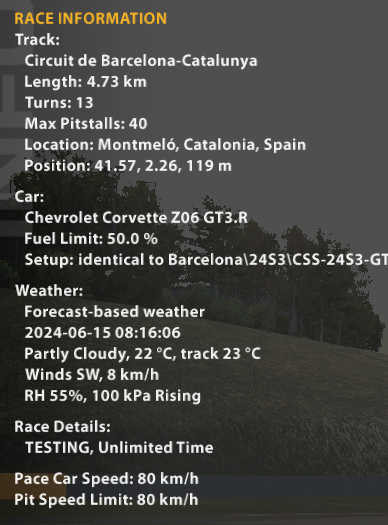
\includegraphics[height=\twosubht]{img/test_1/conditions.png}%
            }\quad
            \subcaptionbox{Иллюстрация прохождения первого поворота на трассе\label{s}}{%
              \includegraphics[height=\twosubht]{img/test_1/cornering.png}%
            }
            
            %\caption{}
            
        \end{figure}
        
        Первый тест состоял из 8 боевых кругов и круга выезда. В начале давление составило 1.65 атм., температуры внутреннего и внешнего слоя FL колеса поддерживались равными $\approx 318$ К. После 8 боевых кругов температура внутреннего слоя составила примерно 367 К, внешнего --- 358 К. 

        Используя нашу формулу с известными радиусами $r_1=0.2286$ м, $r_2=0.3422$, а также приняв $n=0.5$ получим новое давление для четырех колес:
        \begin{gather*}
            p_\text{FL}=1.877, \qquad p_\text{FL}'=1.88,\\
            p_\text{FR}=1.796, \qquad p_\text{FR}'=1.79,\\
            p_\text{RL}=1.874, \qquad p_\text{RL}'=1.88,\\
            p_\text{RR}=1.818, \qquad p_\text{RR}'=1.82.
        \end{gather*}
        Здесь в левом столбце указаны давления, предсказанные нашей формулой, а в правом --- симулятором.

        Как видим, отклонения от показаний симулятора на уровне округления.
    \subsection{Тест 2}
        Второй тест прошел в совершенно других условиях. Была использована другая трасса в очень жаркую погоду (температура трассы составила порядка 48 $\celsius$)

        \begin{figure}[htp]

            % preliminary
            \sbox\twosubbox{%
              \resizebox{\dimexpr.9\linewidth-1em}{!}{%
                \includegraphics[height=4cm]{example-image-a}%
                \includegraphics[height=4cm]{example-image-16x9}%
              }%
            }
            \setlength{\twosubht}{\ht\twosubbox}
            
            % typeset
            
            \centering
            
            \subcaptionbox{Условия на трассе и другая информация\label{f}}{%
              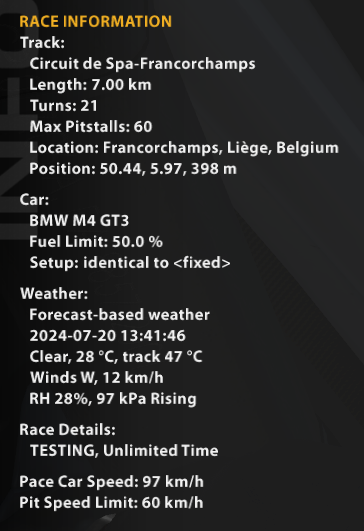
\includegraphics[height=\twosubht]{img/test_2/conditions.png}%
            }\quad
            \subcaptionbox{Вид из кокпита автомобиля на 3 круге\label{s}}{%
              \includegraphics[height=\twosubht]{img/test_2/cornering.png}%
            }
            
            %\caption{}
            
        \end{figure}

        Результаты нашей формулы показаны слева, а показания симулятора --- справа.
        \begin{gather*}
            p_\text{FL}=1.90, \qquad p_\text{FL}'=1.92,\\
            p_\text{FR}=1.92, \qquad p_\text{FR}'=1.92,\\
            p_\text{RL}=1.93, \qquad p_\text{RL}'=1.95,\\
            p_\text{RR}=1.93, \qquad p_\text{RR}'=1.93.
        \end{gather*}
        Как видим, расхождения присутствует с левой стороны, однако они достаточно незначительны.

    \subsection{Тест 3}
        Симулятор позволяет нам моделировать и дождевые условия: они характерны меньшими температурами шин. В этот раз используем другой класс машин, геометрические размеры для этого класса $r_1=0.2286$ м, $r_2=0.3550$ м. Начальное давление равно 1.86 атм.

        \begin{figure}[htp]

            % preliminary
            \sbox\twosubbox{%
              \resizebox{\dimexpr.9\linewidth-1em}{!}{%
                \includegraphics[height=4cm]{example-image-a}%
                \includegraphics[height=4cm]{example-image-16x9}%
              }%
            }
            \setlength{\twosubht}{\ht\twosubbox}
            
            % typeset
            
            \centering
            
            \subcaptionbox{Условия на трассе и другая информация\label{f}}{%
              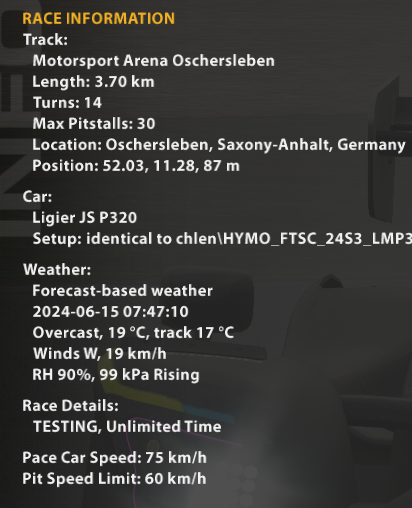
\includegraphics[height=\twosubht]{img/test_3/conditions.png}%
            }\quad
            \subcaptionbox{Иллюстрация прохождения поворота на трассе\label{s}}{%
              \includegraphics[height=\twosubht]{img/test_3/cornering.png}%
            }
            
            %\caption{}
            
        \end{figure}

        С помощью нашей формулы были получены следующие значения (слева), а симулятор показал значения (справа):
        \begin{gather*}
            p_\text{FL}=1.85, \qquad p_\text{FL}'=1.79,\\
            p_\text{FR}=1.84, \qquad p_\text{FR}'=1.79,\\
            p_\text{RL}=1.89, \qquad p_\text{RL}'=1.82,\\
            p_\text{RR}=1.88, \qquad p_\text{RR}'=1.81.
        \end{gather*}
        Как видим, результаты в данном случае довольно сильно различаются. Это может быть связано с слишком маленьким количеством кругов (4), попробуем проехать больше.
        \begin{gather*}
            p_\text{FL}=1.82, \qquad p_\text{FL}'=1.78,\\
            p_\text{FR}=1.81, \qquad p_\text{FR}'=1.77,\\
            p_\text{RL}=1.86, \qquad p_\text{RL}'=1.82,\\
            p_\text{RR}=1.85, \qquad p_\text{RR}'=1.81.
        \end{gather*}
        Как видим, результаты все равно довольно сильно разнятся.

    \section{Другие недостатки нашего результата}
        В целом, формула действительно хорошо себя показала, однако хочется отметить другие ее несовершенства.

        Нам удалось проверить достаточно большой массив разных машин, трасс и условий, чтобы найти все недостатки нашего результата. Мы уже убедились, что она плохо работает в дождевых условиях. Кроме того, в течение тестирования было установлено, что наш результат дает плохое предсказание на машинах, для которых свойственны большие перепады температур. Обычно это более маленькие машины, для которых свойственны микроскольжения, или машины категории открытых колес.
    \section{Влияние степени зависимости коэффициента\\ теплопроводности от температуры}
        При формулировке и решении задачи мы предположили, что $\varkappa \sim T^n$, где $n$ --- произвольный параметр больше нуля. Это несколько усложнило наши вычисления, однако сейчас позволяет нам посмотреть, как он влияет на наши результаты. 

        Рассмотрим, например, RR шину из теста 2. Для нее давление, предсказанное симулятором $p=1.93$ атм, наша же оценка совпала при $n=0.5$. Рассмотрим значения, предсказанные нашей формулой при различных $n$:
        \begin{eqnarray*}
            n=0.5 & \rightarrow & p=1.929,\\
            n=1 & \rightarrow & p=1.930,\\
            n=2 & \rightarrow & p=1.930,\\
            &\dots&\\
            n=10 & \rightarrow & p=1.931.
        \end{eqnarray*}
        Как видим, результат практически не зависит от степени. Даже если поставить $n=0$, то есть $\varkappa=\text{const}$, то получим те же самые $p=1.929$. Это достаточно интересный результат, однако предсказуемый. Диапазон температур, в которых мы работаем слишком мал, чтобы степень $n$ имела большое влияние на результат.
    %\newpage
    \section{Выводы}
        В результате нашей работы мы смогли сформулировать задачу, затем в общем виде (с некоторыми пренебрежениями) решить ее, а затем полученный результат применить на реальных данных.

        Полученный результат довольно хорошо совпадает с результатами симуляции в iRacing. Сервис считается одним из самых точных воспроизведений реальных гоночных характеристик машин, в том числе поведения давления в шинах. К сожалению, сравнить полученный результат с реальностью не представляется возможным, однако мы можем с достаточно высокой точностью подтвердить корректность модели iRacing.

        В ходе проверки результатов были выявлены и недостатки модели: она плохо себя ведет с автомобилями, подверженными более экстремальным перепадам температур в шинах, это также часто вызвано маленькими геометрическими размерами шины.

        Кроме того, наша модель не всегда аккуратно предсказывает давление в дождевых или очень холодных условиях. Это может быть связано с увеличенным влиянием температуры тормозов, а также увеличенным охлаждением внешнего слоя резины. Это создает достаточно высокий градиент температур внутри шины, что влияет на нашу модель в негативном ключе.
    %\end{multicols}

    \begin{thebibliography}{9}
        \bibitem{labnik}
        А.Д. Гладун, Д.А. Александров, Ф.Ф. Игошин, П.Ф. Коротков,
В.П. Корявов, А.П. Овчинников, Ю.А. Самарский, А.А. Теврюков,
Г.Н. Фрейберг \emph{ЛАБОРАТОРНЫЙ
ПРАКТИКУМ
ПО ОБЩЕЙ ФИЗИКЕ}
        \bibitem{sivukhin}
        Д.В.Сивухин
\emph{ОБЩИЙ КУРС ФИЗИКИ.
ТЕРМОДИНАМИКА И МОЛЕКУЛЯРНАЯ ФИЗИКА}
    \end{thebibliography}
\end{document}
